% This is a LaTeX template
% for preparing documents for ITTMM conference

\documentclass[60x84/16,8pt]{ittmm}

% Убедительная просьба к авторам не редактировать файл definition.tex
\usepackage[T1,T2A]{fontenc}
\usepackage{ucs}
\usepackage[utf8x]{inputenc}
\usepackage[english,russian]{babel}

%% Расширенная математика

\usepackage{amsmath}
\usepackage{amssymb}
\usepackage{amscd}

\usepackage{mathtools}
\mathtoolsset{
showonlyrefs=true,
mathic=true,
}

\allowdisplaybreaks

%% Работа с графикой

\usepackage{graphicx}

%% hyperref

\usepackage{hyperref}
\hypersetup{backref,
 colorlinks=false}
\hypersetup{pdfborder=0 0 0}

%% local definitions

\geometry{twoside}
\geometry{bindingoffset=0pt}

\geometry{includehead}
\geometry{hmargin={16mm,16mm},vmargin={12mm,13mm}}
\geometry{marginparwidth=0pt,marginparsep=0pt}
\geometry{headheight=0pt}
\geometry{headsep=\baselineskip}

\pagestyle{empty}

\usepackage{cite}


\begin{document}

% Укажите индекс УДК, соответствующий Вашей работе.
\udc{519.25}

\title{Разработка эффективного алгоритма краткосрочного прогнозирования
  электропотребления с использованием метода ансамбля}

\author[1]{Е. Ю. Щетинин}
\author[2]{М. В. Бережков}
\author[2]{П. Г. Любин}

\address[1]{Всероссийский научно-исследовательский институт\\
  по проблемам гражданской обороны  и чрезвычайных ситуаций\\
  МЧС России (федеральный центр науки и высоких технологий)\\
  ул. Давыдковская, д.7, Москва, Россия, 121352}
\address[2]{Федеральное государственное бюджетное образовательное учреждение\\
  Высшего образования\\
  Московский государственный технологический университет ``СТАНКИН''\\
  пер. Вадковский, д.3а, Москва, Россия, 127055}

\email{\url{lyubin.p@gmail.com}, \url{riviera-molto@mail.ru}}

\begin{abstract}
Краткосрочное прогнозирование потребления электроэнергии является актуальной
задачей во многих областях человеческой деятельности в виду специфичности
продукта: нельзя накопить и хранить энергию впрок. Во-первых,
предприятиям-участникам оптового рынка электроэнергии необходимо заранее
подавать заявки с плановым потреблением, а энергогенерирующим предприятиям
необходимо планировать мощности. Во-вторых, данный показатель может
использоваться в качестве одного из признаков при построение других моделей. При
этом потребление электрической энергии каким-либо объектом является временным
рядом, так как представляет собой мгновенные значения потребляемой мощности
замеренные в различные моменты времени с определенной периодичностью. В данной
работе продемонстрирован простой и эффективный метод краткосрочного
прогнозирования электропотребления. Подход основывается на методе ансамбля
базовых моделей (RPART - Recursive PARTitioning, CTREE - Conditional Inference
Trees \cite{BreimanEtAl}) и имеет хороший уровень прогнозирования, который
сопоставим с более сложными в использовании алгоритмами. Метод ансамбля
представляет собой алгоритм комбинации набора обученных моделей с целью
повышения точности прогноза, но стараясь избежать переобучения. Существует
несколько методов ансамбля, которые имеют свои недостатки и преимущества. В
данной работе мы использовали метод бэггинга (Bagging - Bootstrap aggregating
\cite{Breiman1996}), который помог улучшить прогностическую силу отдельных
базовых моделей.
\end{abstract}

\keywords{краткосрочное прогнозирование, метод ансамбля, RPART, CTREE, 
  случайные деревья, электропотребление, бэггинг}

% \thanks{Рукопись должна содержать УДК, который рекомендуется брать из
%   следующего источника: \url{http://www.mathnet.ru/udc.pdf}.}

\alttitle{Development of an effective algorithm for short-term forecasting of 
  power consumption using ensemble}

\altauthor[1]{E. Yu. Shchetinin}
\altauthor[2]{M. V. Berezhkov}
\altauthor[2]{P. G. Lyubin}

\altaddress[1]{All-Russian Research Institute\\
  for Civil Defense and Emergencies of the MESRF\\
  (Science and High Technology Federal Center)\\
  Davydkovskaya str., 7, Moscow, 121352, Russia}
\altaddress[2]{Moscow State University of Technology ``STANKIN'',\\ 
  Vadkovsky lane, 3a, Moscow, 127055, Russia}

\begin{altabstract}
Short-term forecasting of electricity consumption is an actual task in many
areas of human activity due to the specificity: consumers and power companies
can't accumulate energy and can't store energy. At the first, consumers which
participating in the wholesale electricity market must to submit a plan of
future consumption, and energy-generating companies need to plan the output.
Secondly, this indicator can be used as one of the features when fitting other
models. At the same time, the consumption of electrical energy by any object is
a time series, since it represents the instantaneous values ​​of the consumed
power measured at different times with a certain periodicity. In article we
demonstrate a simple and effective method for short-term forecasting of power
consumption. The approach is based on the method of base models ensemble (RPART
- Recursive PARTitioning, CTREE - Conditional Inference Trees
\cite{BreimanEtAl}) and has a good prediction level comparable with more complex
algorithms. The ensemble method is an algorithm for combining a set of trained
models to improve the accuracy of the forecast with trying to avoid overfitting.
There are several ensemble methods that have their disadvantages and advantages.
We used Bagging (Bootstrap aggregating \cite{Breiman1996}) which helped to
improve the predictive power of particular base models.
\end{altabstract}

\altkeywords{short-term forecast, ensemble, RPART, CTREE, random trees,
  power consumption, bagging}

\maketitle

\section{Введение}
\label{sec:intro}
К наиболее распространенным методам прогнозирования временных рядов относятся:
\begin{itemize}
    \item прогнозная экстраполяция
    \item экспертные (интуитивные) методы прогнозирования
    \item корреляционный и регрессионный анализы
    \item прогнозирование на базе ARIMA моделей
    \item адаптивные методы прогнозирования
    \item прогнозирование с использованием искусственных нейронных сетей
    \item прогнозирование с использованием гибридных сетей
\end{itemize}

Перечисленные методы могут применяться для прогнозирования электропотребления и
обладают присущими им достоинствами и недостатками. В современных работах чаще
остальных описываются решения данной задачи с применением искусственных
нейронных сетей, к недостаткам которых можно отнести сложность настройки и
сложность интерпретации. В данной работе мы используем подход, в котором
используется ансамбль моделей.

На рисунке \ref{fig:data} изображена динамика почасового потребления
электроэнергии в России за 3 недели 2017 года: с 13 июня по 3 июля.
\begin{figure}
  \centering
  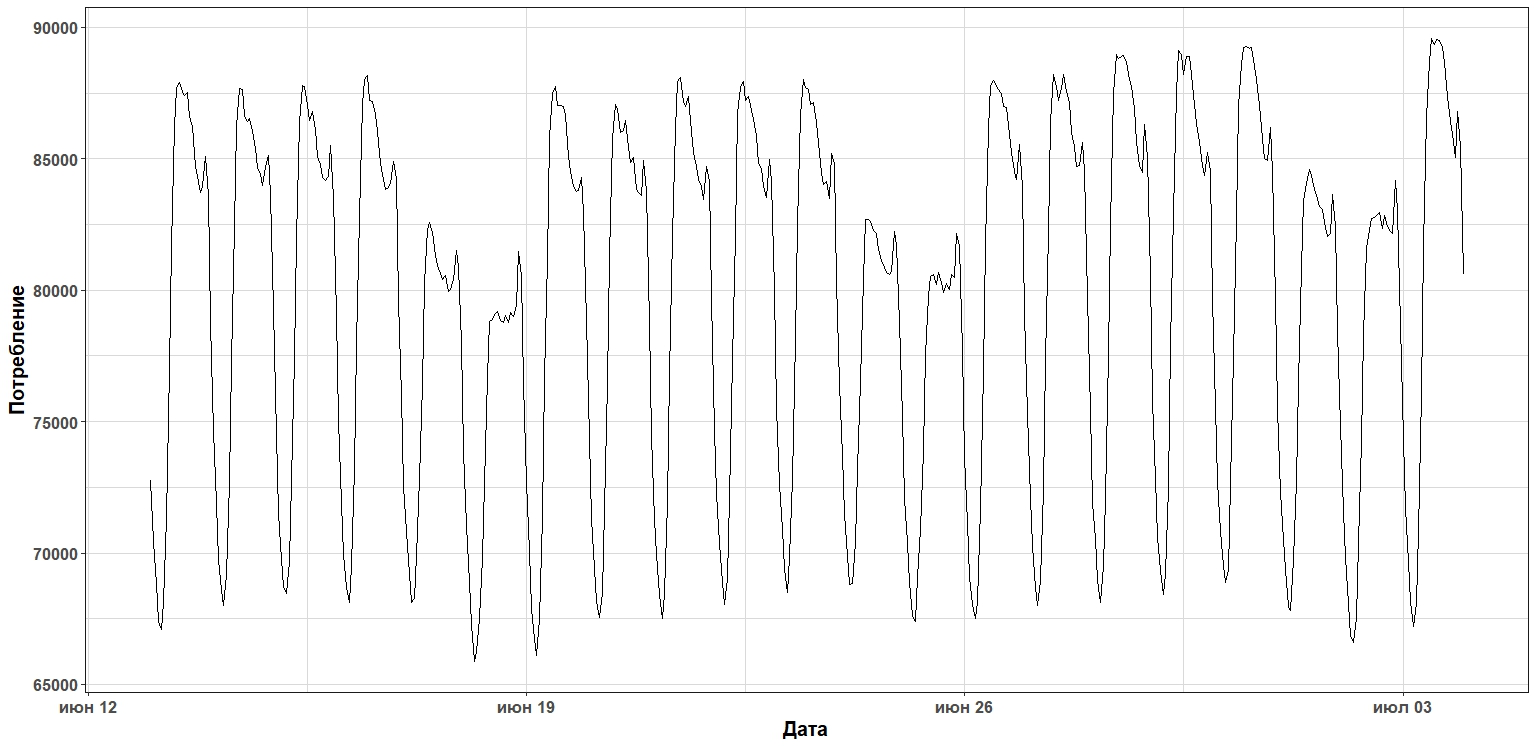
\includegraphics[width=0.6\linewidth]{Ru/train_dataset.jpeg}
  \caption{Исходные данные}
  \label{fig:data}
\end{figure}

\section{Метод}
\label{sec:methods}
К наиболее распространенным методам методам ансамбля относятся:
\begin{itemize}
    \item простое голосование (Simple Voting)
    \item взвешенное голосование (Weighted Voting)
    \item смесь экспертов (Mixture of Experts)
    \item бустинг (Boosting)
    \item бэггинг (Bagging - Bootstrap aggregating \cite{Breiman1996})
\end{itemize}
В своей работе мы использовали бэггинг, который был предложен Л. Брейманом в
1996 году. Суть метода заключается в формировании различных обучающих подвыборок
случайным выбором с возвращениями - некоторые объекты попадают в подвыборку
несколько раз, некоторые ни разу. Базовые алгоритмы, обученные по подвыборкам,
объединяются в композицию с помощью простого голосования. Достоинствами бэггинга
являются: во-первых, возможность использования различных базовых алгоритмов,
ошибки которых могут быть взаимно компенсированы при голосовании; во-вторых,
некоторые обучающие подвыборки могут не содержать объекты-выбросы и алгоритм,
построенный по этим подвыборкам, может оказаться точнее алгоритма, построенного
по полной выборке. В данной работе в качестве базовых алгоритмов используются
RPART и CTREE. Результат прогнозирования потребления электроэнергии на одни
сутки вперед (4 июля 2017 года) приведен на рисунке \ref{fig:prediction}.
\begin{figure}
  \centering
  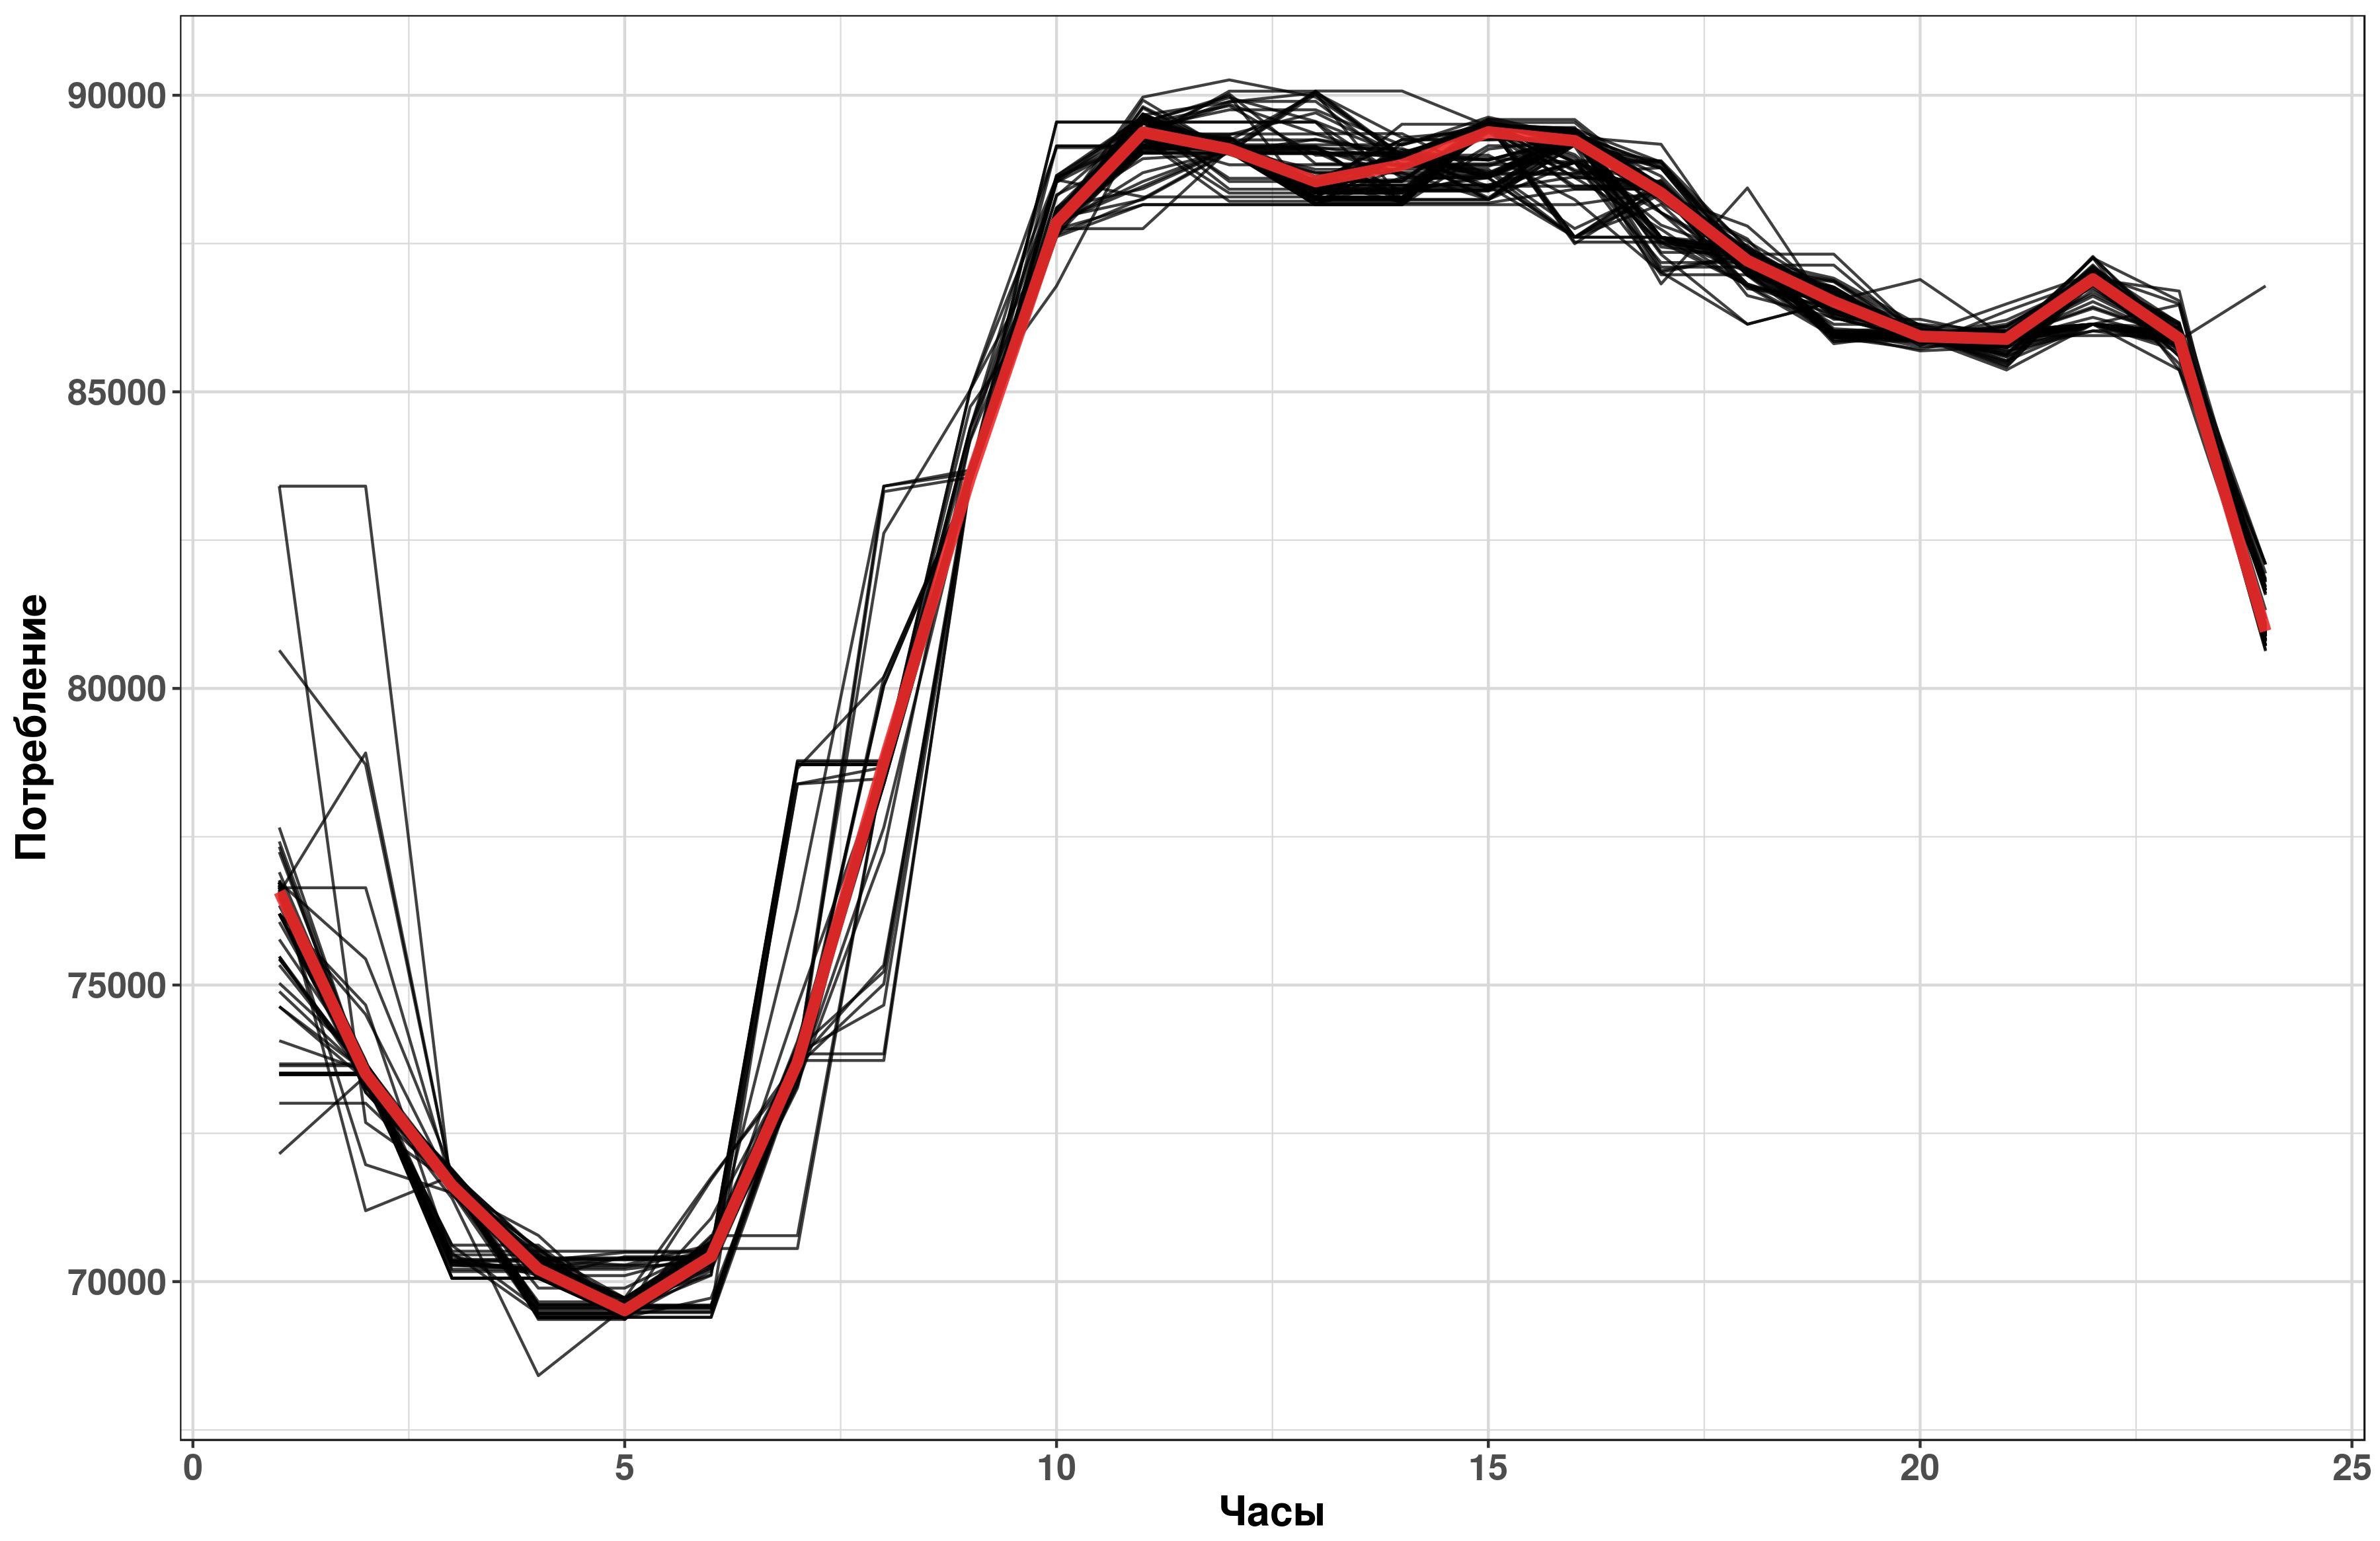
\includegraphics[width=0.6\linewidth]{Ru/prediction.jpg}
  \caption{Прогноз с использованием бэггинга}
  \label{fig:prediction}
\end{figure}


\section{Заключение}
В данной работе продемонстрирован простой и эффективный метод краткосрочного
прогнозирования электропотребления, который может использоваться участниками
рынка энергии при планировании генерации и при планировании закупок.

\begin{thebibliography}{99}

\bibitem{Shetinin}
Е.~Ю. Щетинин, Эффективные компьютерные алгоритмы моделирования спотовых цен на
электроэнергию. - Научное обозрение, 2016. №22, 237-242

\bibitem{ShetininKaplunovMarkov}
Е.~Ю. Щетинин, С.~В. Каплунов, П.~Н. Марков, Моделирование спотовых цен на
электроэнергию с использованием марковских процессов переключения режимов. -
Вестник РУДН, Серия Математика. Информатика. Физика, 2012, №3, 61-68

\bibitem{ShetininLyubin}
Е.~Ю. Щетинин, П.~Г. Любин, Робастный алгоритм построения сглаживающих сплайнов.
- Научное Обозрение, 2015. №1, 86–94

\bibitem{LyubinShetinin}
П.~Г. Любин, Е.~Ю. Щетинин, Стохастические модели сглаживания и прогнозирования
коэффициентов смертности. - Научное Обозрение, 2015, №18, 147–155

\bibitem{BreimanEtAl}
L. Breiman, J.~H. Friedman, R.~A. Olshen, C.~J. Stone, Classification and
Regression Trees. - Wadsworth, California.

\bibitem{Breiman1996}
L. Breiman, Bagging Predictors. - Machine Learning, 1996, 24, 123-140

\end{thebibliography}


% % Возможно использовать bibtex.
% \bibliographystyle{elsarticle-num}
% \bibliography{ittmm-template-ru}


\makealttitle      

\end{document}
